\section{5. 有向树与有序树}
\begin{frame}
  \frametitle{5. 有向树与有序树}
  \begin{Def}
    一个有向图,如果抹去其所有弧的方向以后所得到的无向图是一棵无向树,则称该有向图为一棵\alert{有向树}。
  \end{Def}
\end{frame}
\begin{frame}
  \centering
\begin{minipage}{0.24\linewidth}\centering
  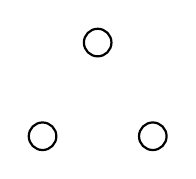
\begin{tikzpicture}[auto,
    specification/.style ={circle, draw, thick,inner sep=0pt, minimum size=5mm,scale = 0.7},scale = 0.7]
   \node[specification] (A)  at (-1,0)  {};
   \node[specification] (B)  at (1,0)  {};
   \node[specification] (C)  at (0,1.7)  {};
 \end{tikzpicture}\\
  A
\end{minipage}\hfill
\begin{minipage}{0.24\linewidth}\centering
  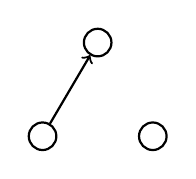
\begin{tikzpicture}[auto,
    specification/.style ={circle, draw, thick,inner sep=0pt, minimum size=5mm,scale = 0.7},scale = 0.7]
   \node[specification] (A)  at (-1,0)  {};
   \node[specification] (B)  at (1,0)  {};
   \node[specification] (C)  at (0,1.7)  {};
   \draw[thick, ->] (A) to  (C);
 \end{tikzpicture}\\
B
\end{minipage}\hfill
 \begin{minipage}{0.24\linewidth}\centering
  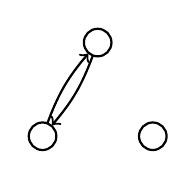
\begin{tikzpicture}[auto,
    specification/.style ={circle, draw, thick,inner sep=0pt, minimum size=5mm,scale = 0.7},scale = 0.7]
   \node[specification] (A)  at (-1,0)  {};
   \node[specification] (B)  at (1,0)  {};
   \node[specification] (C)  at (0,1.7)  {};
   \draw[thick, ->] (A) to  [bend left=10] (C);
   \draw[thick, ->] (C) to  [bend left=10] (A);   
 \end{tikzpicture}\\
C
\end{minipage}\hfill
 \begin{minipage}{0.24\linewidth}\centering
  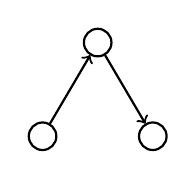
\begin{tikzpicture}[auto,
    specification/.style ={circle, draw, thick,inner sep=0pt, minimum size=5mm,scale = 0.7},scale = 0.7]
   \node[specification] (A)  at (-1,0)  {};
   \node[specification] (B)  at (1,0)  {};
   \node[specification] (C)  at (0,1.7)  {};
   \draw[thick, ->] (A) to  (C);
   \draw[thick, ->] (C) to  (B);
 \end{tikzpicture}\\
D
\end{minipage}

\vspace{0.3cm}
 \begin{minipage}{0.24\linewidth}\centering
  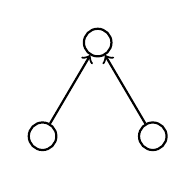
\begin{tikzpicture}[auto,
    specification/.style ={circle, draw, thick,inner sep=0pt, minimum size=5mm,scale = 0.7},scale = 0.7]
   \node[specification] (A)  at (-1,0)  {};
   \node[specification] (B)  at (1,0)  {};
   \node[specification] (C)  at (0,1.7)  {};
   \draw[thick, ->] (A) to  (C);
   \draw[thick, ->] (B) to  (C);
\end{tikzpicture}\\
  E
\end{minipage}\hfill
 \begin{minipage}{0.24\linewidth}\centering
  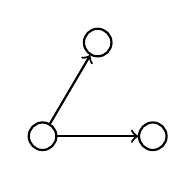
\begin{tikzpicture}[auto,
    specification/.style ={circle, draw, thick,inner sep=0pt, minimum size=5mm,scale = 0.7},scale = 0.7]
   \node[specification] (A)  at (-1,0)  {};
   \node[specification] (B)  at (1,0)  {};
   \node[specification] (C)  at (0,1.7)  {};
   \draw[thick, ->] (A) to  (C);
   \draw[thick, ->] (A) to  (B);
\end{tikzpicture}\\
  F
\end{minipage}\hfill
 \begin{minipage}{0.24\linewidth}\centering
  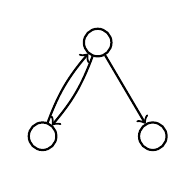
\begin{tikzpicture}[auto,
    specification/.style ={circle, draw, thick,inner sep=0pt, minimum size=5mm,scale = 0.7},scale = 0.7]
   \node[specification] (A)  at (-1,0)  {};
   \node[specification] (B)  at (1,0)  {};
   \node[specification] (C)  at (0,1.7)  {};
   \draw[thick, ->] (A) to  [bend left=10] (C);
   \draw[thick, ->] (C) to  [bend left=10] (A);
   \draw[thick, ->] (C) to  (B);   
\end{tikzpicture}\\
  G
\end{minipage}\hfill
 \begin{minipage}{0.24\linewidth}\centering
  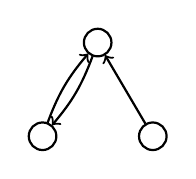
\begin{tikzpicture}[auto,
    specification/.style ={circle, draw, thick,inner sep=0pt, minimum size=5mm,scale = 0.7},scale = 0.7]
   \node[specification] (A)  at (-1,0)  {};
   \node[specification] (B)  at (1,0)  {};
   \node[specification] (C)  at (0,1.7)  {};
   \draw[thick, ->] (A) to  [bend left=10] (C);
   \draw[thick, ->] (C) to  [bend left=10] (A);
   \draw[thick, ->] (B) to  (C);
 \end{tikzpicture}\\
  H
\end{minipage}

\vspace{0.3cm}
 \begin{minipage}{0.24\linewidth}\centering
  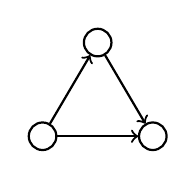
\begin{tikzpicture}[auto,
    specification/.style ={circle, draw, thick,inner sep=0pt, minimum size=5mm,scale = 0.7},scale = 0.7]
   \node[specification] (A)  at (-1,0)  {};
   \node[specification] (B)  at (1,0)  {};
   \node[specification] (C)  at (0,1.7)  {};
   \draw[thick, ->] (A) to  (C);
   \draw[thick, ->] (C) to  (B);
   \draw[thick, ->] (A) to  (B);   
\end{tikzpicture}\\
  I
\end{minipage}\hfill
 \begin{minipage}{0.24\linewidth}\centering
  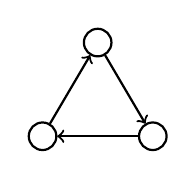
\begin{tikzpicture}[auto,
    specification/.style ={circle, draw, thick,inner sep=0pt, minimum size=5mm,scale = 0.7},scale = 0.7]
   \node[specification] (A)  at (-1,0)  {};
   \node[specification] (B)  at (1,0)  {};
   \node[specification] (C)  at (0,1.7)  {};
   \draw[thick, ->] (A) to  (C);
   \draw[thick, ->] (C) to  (B);
   \draw[thick, ->] (B) to  (A);
 \end{tikzpicture}\\
  J
\end{minipage}\hfill
 \begin{minipage}{0.24\linewidth}\centering
  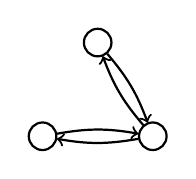
\begin{tikzpicture}[auto,
    specification/.style ={circle, draw, thick,inner sep=0pt, minimum size=5mm,scale = 0.7},scale = 0.7]
   \node[specification] (A)  at (-1,0)  {};
   \node[specification] (B)  at (1,0)  {};
   \node[specification] (C)  at (0,1.7)  {};
   \draw[thick, ->] (A) to  [bend left=10] (B);
   \draw[thick, ->] (B) to  [bend left=10] (A);
   \draw[thick, ->] (B) to  [bend left=10] (C);
   \draw[thick, ->] (C) to  [bend left=10] (B);
 \end{tikzpicture}\\
  K
\end{minipage}\hfill
 \begin{minipage}{0.24\linewidth}\centering
  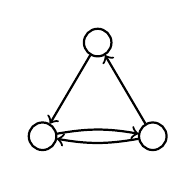
\begin{tikzpicture}[auto,
    specification/.style ={circle, draw, thick,inner sep=0pt, minimum size=5mm,scale = 0.7},scale = 0.7]
   \node[specification] (A)  at (-1,0)  {};
   \node[specification] (B)  at (1,0)  {};
   \node[specification] (C)  at (0,1.7)  {};
   \draw[thick, ->] (A) to  [bend left=10] (B);
   \draw[thick, ->] (B) to  [bend left=10] (A);
   \draw[thick, ->] (B) to  (C);
   \draw[thick, ->] (C) to  (A);
 \end{tikzpicture}\\
  L
\end{minipage}

\vspace{0.3cm}
 \begin{minipage}{0.24\linewidth}\centering
   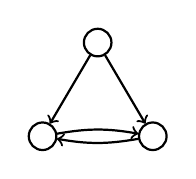
\begin{tikzpicture}[auto,
    specification/.style ={circle, draw, thick,inner sep=0pt, minimum size=5mm,scale = 0.7},scale = 0.7]
   \node[specification] (A)  at (-1,0)  {};
   \node[specification] (B)  at (1,0)  {};
   \node[specification] (C)  at (0,1.7)  {};
   \draw[thick, ->] (A) to  [bend left=10] (B);
   \draw[thick, ->] (B) to  [bend left=10] (A);
   \draw[thick, ->] (C) to  (B);
   \draw[thick, ->] (C) to  (A);
 \end{tikzpicture}\\
  M
\end{minipage}\hfill
 \begin{minipage}{0.24\linewidth}\centering
  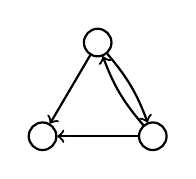
\begin{tikzpicture}[auto,
    specification/.style ={circle, draw, thick,inner sep=0pt, minimum size=5mm,scale = 0.7},scale = 0.7]
   \node[specification] (A)  at (-1,0)  {};
   \node[specification] (B)  at (1,0)  {};
   \node[specification] (C)  at (0,1.7)  {};
   \draw[thick, ->] (C) to   (A);
   \draw[thick, ->] (B) to   (A);
   \draw[thick, ->] (B) to  [bend left=10] (C);
   \draw[thick, ->] (C) to  [bend left=10] (B);
 \end{tikzpicture}\\
  N
\end{minipage}\hfill
 \begin{minipage}{0.24\linewidth}\centering
  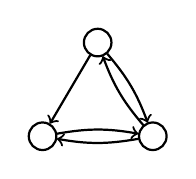
\begin{tikzpicture}[auto,
    specification/.style ={circle, draw, thick,inner sep=0pt, minimum size=5mm,scale = 0.7},scale = 0.7]
   \node[specification] (A)  at (-1,0)  {};
   \node[specification] (B)  at (1,0)  {};
   \node[specification] (C)  at (0,1.7)  {};
   \draw[thick, ->] (A) to  [bend left=10] (B);
   \draw[thick, ->] (B) to  [bend left=10] (A);
   \draw[thick, ->] (B) to  [bend left=10] (C);
   \draw[thick, ->] (C) to  [bend left=10] (B);
   \draw[thick, ->] (C) to   (A);   
 \end{tikzpicture}\\
  O
\end{minipage}\hfill
 \begin{minipage}{0.24\linewidth}\centering
  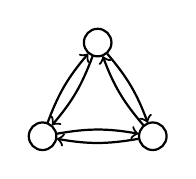
\begin{tikzpicture}[auto,
    specification/.style ={circle, draw, thick,inner sep=0pt, minimum size=5mm,scale = 0.7},scale = 0.7]
   \node[specification] (A)  at (-1,0)  {};
   \node[specification] (B)  at (1,0)  {};
   \node[specification] (C)  at (0,1.7)  {};
   \draw[thick, ->] (A) to  [bend left=10] (B);
   \draw[thick, ->] (B) to  [bend left=10] (A);
   \draw[thick, ->] (B) to  [bend left=10] (C);
   \draw[thick, ->] (C) to  [bend left=10] (B);
   \draw[thick, ->] (A) to  [bend left=10] (C);
   \draw[thick, ->] (C) to  [bend left=10] (A);   
 \end{tikzpicture}\\
  P
\end{minipage}
\end{frame}

\begin{frame}
  \frametitle{5. 有向树与有序树}
  \begin{Def}
    有向树$D$称为\alert{有根树},如果$D$中恰有一个顶点的入度为0,而其余每个顶点的入度均为1。有根树中入度为0的顶点称为有根树的根,出度为0的顶点称为\alert{叶子},非叶顶点称为\alert{分支点}或\alert{内顶点}。
  \end{Def}
\end{frame}
\begin{frame}
  \centering
\begin{minipage}{0.24\linewidth}\centering
  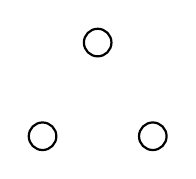
\begin{tikzpicture}[auto,
    specification/.style ={circle, draw, thick,inner sep=0pt, minimum size=5mm,scale = 0.7},scale = 0.7]
   \node[specification] (A)  at (-1,0)  {};
   \node[specification] (B)  at (1,0)  {};
   \node[specification] (C)  at (0,1.7)  {};
 \end{tikzpicture}\\
  A
\end{minipage}\hfill
\begin{minipage}{0.24\linewidth}\centering
  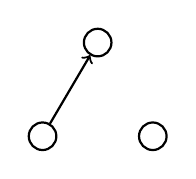
\begin{tikzpicture}[auto,
    specification/.style ={circle, draw, thick,inner sep=0pt, minimum size=5mm,scale = 0.7},scale = 0.7]
   \node[specification] (A)  at (-1,0)  {};
   \node[specification] (B)  at (1,0)  {};
   \node[specification] (C)  at (0,1.7)  {};
   \draw[thick, ->] (A) to  (C);
 \end{tikzpicture}\\
B
\end{minipage}\hfill
 \begin{minipage}{0.24\linewidth}\centering
  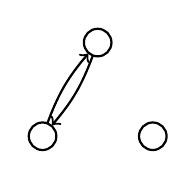
\begin{tikzpicture}[auto,
    specification/.style ={circle, draw, thick,inner sep=0pt, minimum size=5mm,scale = 0.7},scale = 0.7]
   \node[specification] (A)  at (-1,0)  {};
   \node[specification] (B)  at (1,0)  {};
   \node[specification] (C)  at (0,1.7)  {};
   \draw[thick, ->] (A) to  [bend left=10] (C);
   \draw[thick, ->] (C) to  [bend left=10] (A);   
 \end{tikzpicture}\\
C
\end{minipage}\hfill
 \begin{minipage}{0.24\linewidth}\centering
  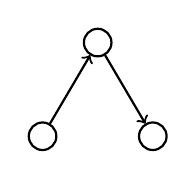
\begin{tikzpicture}[auto,
    specification/.style ={circle, draw, thick,inner sep=0pt, minimum size=5mm,scale = 0.7},scale = 0.7]
   \node[specification] (A)  at (-1,0)  {};
   \node[specification] (B)  at (1,0)  {};
   \node[specification] (C)  at (0,1.7)  {};
   \draw[thick, ->] (A) to  (C);
   \draw[thick, ->] (C) to  (B);
 \end{tikzpicture}\\
D
\end{minipage}

\vspace{0.3cm}
 \begin{minipage}{0.24\linewidth}\centering
  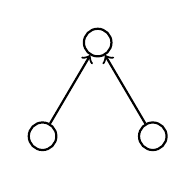
\begin{tikzpicture}[auto,
    specification/.style ={circle, draw, thick,inner sep=0pt, minimum size=5mm,scale = 0.7},scale = 0.7]
   \node[specification] (A)  at (-1,0)  {};
   \node[specification] (B)  at (1,0)  {};
   \node[specification] (C)  at (0,1.7)  {};
   \draw[thick, ->] (A) to  (C);
   \draw[thick, ->] (B) to  (C);
\end{tikzpicture}\\
  E
\end{minipage}\hfill
 \begin{minipage}{0.24\linewidth}\centering
  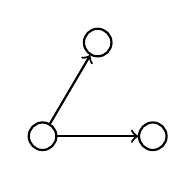
\begin{tikzpicture}[auto,
    specification/.style ={circle, draw, thick,inner sep=0pt, minimum size=5mm,scale = 0.7},scale = 0.7]
   \node[specification] (A)  at (-1,0)  {};
   \node[specification] (B)  at (1,0)  {};
   \node[specification] (C)  at (0,1.7)  {};
   \draw[thick, ->] (A) to  (C);
   \draw[thick, ->] (A) to  (B);
\end{tikzpicture}\\
  F
\end{minipage}\hfill
 \begin{minipage}{0.24\linewidth}\centering
  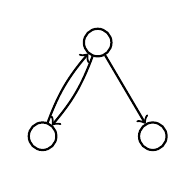
\begin{tikzpicture}[auto,
    specification/.style ={circle, draw, thick,inner sep=0pt, minimum size=5mm,scale = 0.7},scale = 0.7]
   \node[specification] (A)  at (-1,0)  {};
   \node[specification] (B)  at (1,0)  {};
   \node[specification] (C)  at (0,1.7)  {};
   \draw[thick, ->] (A) to  [bend left=10] (C);
   \draw[thick, ->] (C) to  [bend left=10] (A);
   \draw[thick, ->] (C) to  (B);   
\end{tikzpicture}\\
  G
\end{minipage}\hfill
 \begin{minipage}{0.24\linewidth}\centering
  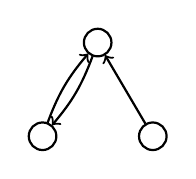
\begin{tikzpicture}[auto,
    specification/.style ={circle, draw, thick,inner sep=0pt, minimum size=5mm,scale = 0.7},scale = 0.7]
   \node[specification] (A)  at (-1,0)  {};
   \node[specification] (B)  at (1,0)  {};
   \node[specification] (C)  at (0,1.7)  {};
   \draw[thick, ->] (A) to  [bend left=10] (C);
   \draw[thick, ->] (C) to  [bend left=10] (A);
   \draw[thick, ->] (B) to  (C);
 \end{tikzpicture}\\
  H
\end{minipage}

\vspace{0.3cm}
 \begin{minipage}{0.24\linewidth}\centering
  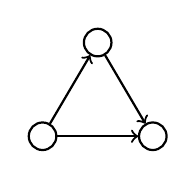
\begin{tikzpicture}[auto,
    specification/.style ={circle, draw, thick,inner sep=0pt, minimum size=5mm,scale = 0.7},scale = 0.7]
   \node[specification] (A)  at (-1,0)  {};
   \node[specification] (B)  at (1,0)  {};
   \node[specification] (C)  at (0,1.7)  {};
   \draw[thick, ->] (A) to  (C);
   \draw[thick, ->] (C) to  (B);
   \draw[thick, ->] (A) to  (B);   
\end{tikzpicture}\\
  I
\end{minipage}\hfill
 \begin{minipage}{0.24\linewidth}\centering
  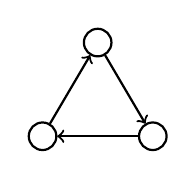
\begin{tikzpicture}[auto,
    specification/.style ={circle, draw, thick,inner sep=0pt, minimum size=5mm,scale = 0.7},scale = 0.7]
   \node[specification] (A)  at (-1,0)  {};
   \node[specification] (B)  at (1,0)  {};
   \node[specification] (C)  at (0,1.7)  {};
   \draw[thick, ->] (A) to  (C);
   \draw[thick, ->] (C) to  (B);
   \draw[thick, ->] (B) to  (A);
 \end{tikzpicture}\\
  J
\end{minipage}\hfill
 \begin{minipage}{0.24\linewidth}\centering
  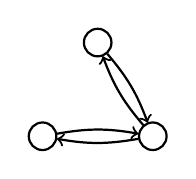
\begin{tikzpicture}[auto,
    specification/.style ={circle, draw, thick,inner sep=0pt, minimum size=5mm,scale = 0.7},scale = 0.7]
   \node[specification] (A)  at (-1,0)  {};
   \node[specification] (B)  at (1,0)  {};
   \node[specification] (C)  at (0,1.7)  {};
   \draw[thick, ->] (A) to  [bend left=10] (B);
   \draw[thick, ->] (B) to  [bend left=10] (A);
   \draw[thick, ->] (B) to  [bend left=10] (C);
   \draw[thick, ->] (C) to  [bend left=10] (B);
 \end{tikzpicture}\\
  K
\end{minipage}\hfill
 \begin{minipage}{0.24\linewidth}\centering
  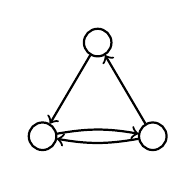
\begin{tikzpicture}[auto,
    specification/.style ={circle, draw, thick,inner sep=0pt, minimum size=5mm,scale = 0.7},scale = 0.7]
   \node[specification] (A)  at (-1,0)  {};
   \node[specification] (B)  at (1,0)  {};
   \node[specification] (C)  at (0,1.7)  {};
   \draw[thick, ->] (A) to  [bend left=10] (B);
   \draw[thick, ->] (B) to  [bend left=10] (A);
   \draw[thick, ->] (B) to  (C);
   \draw[thick, ->] (C) to  (A);
 \end{tikzpicture}\\
  L
\end{minipage}

\vspace{0.3cm}
 \begin{minipage}{0.24\linewidth}\centering
   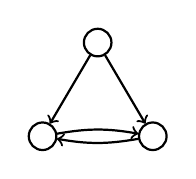
\begin{tikzpicture}[auto,
    specification/.style ={circle, draw, thick,inner sep=0pt, minimum size=5mm,scale = 0.7},scale = 0.7]
   \node[specification] (A)  at (-1,0)  {};
   \node[specification] (B)  at (1,0)  {};
   \node[specification] (C)  at (0,1.7)  {};
   \draw[thick, ->] (A) to  [bend left=10] (B);
   \draw[thick, ->] (B) to  [bend left=10] (A);
   \draw[thick, ->] (C) to  (B);
   \draw[thick, ->] (C) to  (A);
 \end{tikzpicture}\\
  M
\end{minipage}\hfill
 \begin{minipage}{0.24\linewidth}\centering
  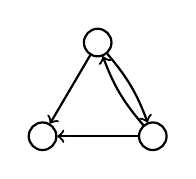
\begin{tikzpicture}[auto,
    specification/.style ={circle, draw, thick,inner sep=0pt, minimum size=5mm,scale = 0.7},scale = 0.7]
   \node[specification] (A)  at (-1,0)  {};
   \node[specification] (B)  at (1,0)  {};
   \node[specification] (C)  at (0,1.7)  {};
   \draw[thick, ->] (C) to   (A);
   \draw[thick, ->] (B) to   (A);
   \draw[thick, ->] (B) to  [bend left=10] (C);
   \draw[thick, ->] (C) to  [bend left=10] (B);
 \end{tikzpicture}\\
  N
\end{minipage}\hfill
 \begin{minipage}{0.24\linewidth}\centering
  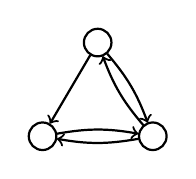
\begin{tikzpicture}[auto,
    specification/.style ={circle, draw, thick,inner sep=0pt, minimum size=5mm,scale = 0.7},scale = 0.7]
   \node[specification] (A)  at (-1,0)  {};
   \node[specification] (B)  at (1,0)  {};
   \node[specification] (C)  at (0,1.7)  {};
   \draw[thick, ->] (A) to  [bend left=10] (B);
   \draw[thick, ->] (B) to  [bend left=10] (A);
   \draw[thick, ->] (B) to  [bend left=10] (C);
   \draw[thick, ->] (C) to  [bend left=10] (B);
   \draw[thick, ->] (C) to   (A);   
 \end{tikzpicture}\\
  O
\end{minipage}\hfill
 \begin{minipage}{0.24\linewidth}\centering
  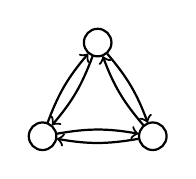
\begin{tikzpicture}[auto,
    specification/.style ={circle, draw, thick,inner sep=0pt, minimum size=5mm,scale = 0.7},scale = 0.7]
   \node[specification] (A)  at (-1,0)  {};
   \node[specification] (B)  at (1,0)  {};
   \node[specification] (C)  at (0,1.7)  {};
   \draw[thick, ->] (A) to  [bend left=10] (B);
   \draw[thick, ->] (B) to  [bend left=10] (A);
   \draw[thick, ->] (B) to  [bend left=10] (C);
   \draw[thick, ->] (C) to  [bend left=10] (B);
   \draw[thick, ->] (A) to  [bend left=10] (C);
   \draw[thick, ->] (C) to  [bend left=10] (A);   
 \end{tikzpicture}\\
  P
\end{minipage}
\end{frame}

\begin{frame}
  \frametitle{5. 有向树与有序树}
  \begin{Def}
  设$T=(V,A)$为一棵有根树。如果$(u,v)\in A$,则称$v$为$u$的\alert{儿子},$u$为$v$的\alert{父亲}。如果从顶点$u$能达到顶点$v$,则称$v$为$u$的\alert{子孙},$u$为$v$的\alert{祖先}。如果$u$是$v$的祖先且$u \neq v$,则称$u$为$v$的\alert{真祖先},$v$为$u$的\alert{真子孙}。
  \end{Def}
\end{frame}

\begin{frame}
  \frametitle{5. 有向树与有序树}
  \begin{Def}\justifying\let\raggedright\justifying
    设$T=(V,A)$为一棵以$v_0$为根的有根树。从$v_0$到顶点$v$的有向路的长度称为$T$的顶点$v$的\alert{深度}。从顶点$v$到$T$的叶子的最长的有向路的长度称为顶点$v$在$T$中的\alert{高度}。根顶点$v_0$的高度称为树$T$的\alert{高度}。
  \end{Def}
\end{frame}

\begin{frame}
  \frametitle{5. 有向树与有序树}
  \begin{Def}
    设$T=(V,A)$为一棵有根树,$v$是$T$的一个顶点,由$v$及其子孙所导出的$T$的子图称为$T$的以$v$为根的\alert{子树}。
  \end{Def}
\end{frame}

\begin{frame}
  \frametitle{5. 有向树与有序树}
  \begin{Def}
    设$T=(V,A)$为一棵有根树。如果$T$的每个顶点的各个儿子排定了次序,则称$T$为一
    棵\alert{有序树}。
  \end{Def}
\end{frame}

\begin{frame}
  \frametitle{5. 有向树与有序树}
  \begin{Def}
    有序树$T$称为\alert{$m$元有序树},如果$T$的每个顶点的出度$\leq m$。一棵$m$元
    有序树$T$称为\alert{正则$m$元有序树},如果$T$的每个顶点的出度不是$0$就是$m$。
    二元有序树简称\alert{二元树}。
  \end{Def}
\end{frame}

%%% Local Variables:
%%% mode: latex
%%% TeX-master: "chapter10"
%%% End:
